\documentclass[20pt]{article}
\usepackage[utf8]{inputenc}
\usepackage{amsmath, amssymb, amsthm}
\usepackage{titlesec}
\usepackage{pgfplots}
\usepackage{graphicx}
% Customization -------

% Paper size, margin
\usepackage[letterpaper,top=1.5cm,bottom=1.5cm,left=1.75cm,right=1.75cm,heightrounded]{geometry}

% line height
\renewcommand{\baselinestretch}{1.15} % line space

% Paragraph indentation 
\setlength{\parindent}{0pt} % no indent

% Paragraph spacing
\setlength{\parskip}{0.8em} % space between paragraphs

% Section number formatting
\titleformat{\section}[hang]{\bfseries}{Problem \thesection\ }{0pt}{}


% Equation numbering per section
\counterwithin*{equation}{section}
\counterwithin*{equation}{subsection}

% Graphics path
\graphicspath{ {./images/} }

% --------------------

\title{ECE421: Assignment 03}
\author{Farbod Mohammadzadeh\\
    1008360462}
\date{11 October 2023}

\begin{document}
\Large


\maketitle

\newpage

\section{}

\subsection*{\underline{Part 1:}}

Points:

\begin{eqnarray}
    x^{(1)} =  \begin{bmatrix}
        1 \\
        1
    \end{bmatrix},
    x^{(2)} = \begin{bmatrix}
        -1 \\
        -1
    \end{bmatrix},
    x^{(3)} = \begin{bmatrix}
        1 \\
        0
    \end{bmatrix},
    x^{(4)} = \begin{bmatrix}
        0 \\
        1
    \end{bmatrix} \\
    t^{(1)} = 1, t^{(2)} = -1, t^{(3)} = -1, t^{(4)} = -1
\end{eqnarray}

Graph:
\begin{figure}[h]
    \centering
    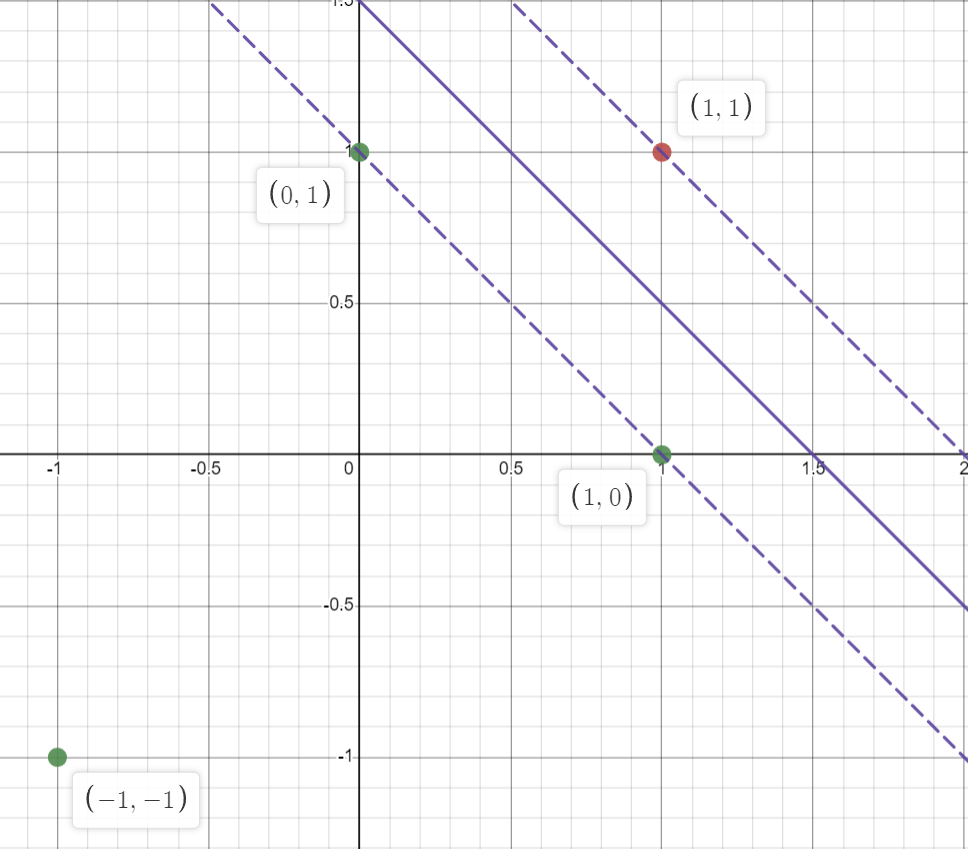
\includegraphics[width=10cm]{desmos-graph}
    \caption{Plot of the points}
    \label{fig:points}
\end{figure}

The equation for the decision boundary is: $y\ =\ -x+1.5$. And the equation for the margins are: $y\ =\ -x+1.5 \pm0.5$.

\subsection*{\underline{Part 2:}}

From the above figure \ref{fig:points}, we can see that the support vectors are $x^{(1)}$, $x^{(3)}$, and $x^{(4)}$.

\subsection*{\underline{Part 3:}}



\end{document}